\chapter{Methodology}
\label{chap:2}
\ChapterPageStuff{2}

\section{Preamble}

\section{Logging mechanism}\label{Ch2:LoggingMechanism} The logging mechanism will need to meet the requirements discussed in \Cref{sec:EventLogging} to capture the required logs to apply system utilisation analysis on it. \Cref{fig:CH2_SystemA_Arch_Design} is the design for the logging mechanism to capture the user's activities. In this figure the logging mechanism is split up into two functional requirements parts (\textbf{F/R}) which consist of the client and server functional requirements.\par Each functional requirements has interface requirement with each other to transfer any of the required data or start a process in another functional requirements. These interfaces are labelled as \textbf{I/F} in \Cref{fig:CH2_SystemA_Arch_Design}.

\begin{figure}[!htb] % An h :here, t: top, b: bottom.
	\centering % cent the figure
	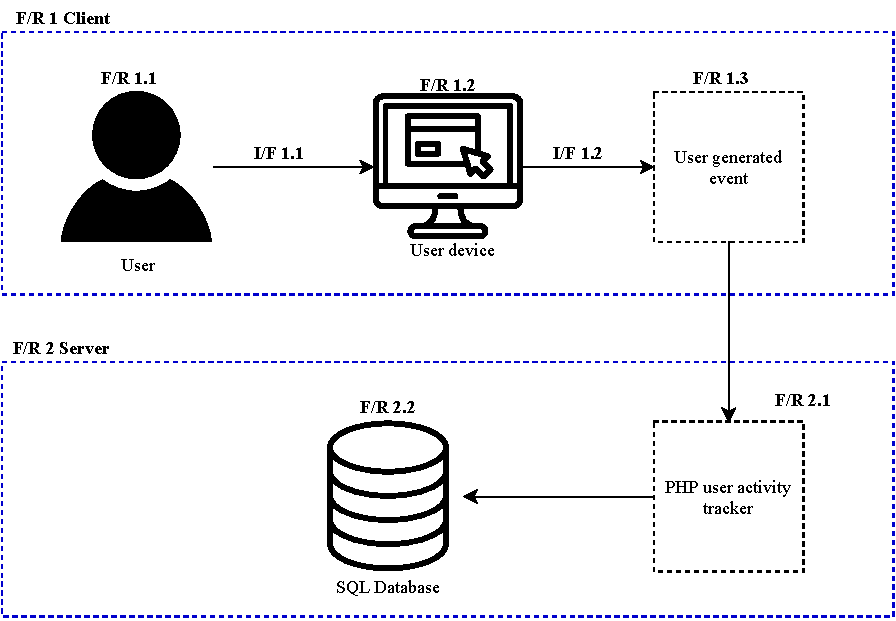
\includegraphics[width=0.9\textwidth]{Chapter2/SystemA_Architecture_Diagram/SystemA_Architecture_Diagram.pdf}
	\caption[System A logging mechanism architecture design]
	{\textit{System A logging mechanism architecture design}}\label{fig:CH2_SystemA_Arch_Design}
\end{figure}

The client's functional requirements (F/R 1) consist of the user interacting with a device on website. In \Cref{tbl:Ch2_Client_Functional_Requirements} is the functional requirements that is on the client side of the user activity logging mechanism.

\begin{table}[!htb]
	\centering
	\small
	\caption[Client functional requirements]
	{\textit{Client functional requirements (F/R 1)}}
	\label{tbl:Ch2_Client_Functional_Requirements}
	\begin{tabularx}{\textwidth}{|l|l|X|}
		\hline \textbf{Requirement ID} & \textbf{Name} & \textbf{Description} \\
		\hline F/R 1.1 & User & The user serves as primary initiator of the activity events.\\
		\hline F/R 1.2 & User's device & The device that user uses to access the website from where the activity events are generated.\\
		\hline F/R 1.3 & User generated events & These are any activity events that user started that needs to communicate back to server.\\
		\hline
	\end{tabularx}
\end{table}

The functional requirements in \Cref{tbl:Ch2_Client_Functional_Requirements} needs to interface with each other.

\begin{table}[!htb]
	\centering
	\small
	\caption[Client interface requirements]
	{\textit{Client interface requirements for F/R 1.1}}
	\label{tbl:Ch2_Client_Interface_Requirements}
	\begin{tabularx}{\textwidth}{|l|l|X|}
		\hline \textbf{Requirement ID} & \textbf{Name} & \textbf{Description} \\
		\hline I/F 1.1 & User input & The user starts the activity events by using the user interface to give the website any input.\\
		\hline I/F 1.2 & Log parsing of logging points & Some of the key logging points can be identified at this point of some of the basic event log attributes in \Cref{tbl:CH1_Log_Basic_Attributes}.\\
		\hline F/R 1.3 & User generated events & These are any activity events that user started that needs to communicate back to server.\\
		\hline
	\end{tabularx}
\end{table}

\section{System utilisation analysis}

\section{integration}

\section{Conclusion}